%
% overview.tex
%
% Copyright (C) 2015, Achim Lösch <achim.loesch@upb.de>, Christoph Knorr <cknorr@mail.uni-paderborn.de>
% All rights reserved.
%
% This documentation may be modified and distributed under the terms
% of the BSD license. See the LICENSE file for details.
%
% encoding: UTF-8
% tab size: 4
%
% author: Achim Lösch (achim.loesch@upb.de)
% created: 7/24/14
% version: 0.5.8 - change project name to ampehre
%

\section{User Manual}\label{sec:UserManual}
MSMonitor is a tool to measure and monitor the power consumption as well as the temperature of hetorgeneous nodes. This version features a client/server implementation, which enables a more precise and efficient measurement.
In the following the client and server options are to be explained. 

\subsection{Server}
The server is supposed to run on the heterogenous node itself, in order to measure the needed information. It awaits incoming requests and responds to them, so the server program is a pure command line application with the following two options:\newline
\begin{center}
	\begin{tabularx}{.9\textwidth}{|>{\hsize=.36\textwidth}X|X|}
		\hline
		\textbf{Option} & \textbf{Description} \\ \hline
		-p & specifies the port which the server listens to for any requests. This port has to be equally chosen on the client\\ \hline
		-d & enables a debug mode with verbose output\\ \hline
	\end{tabularx}
\end{center}
The server is capable of supplying up to 5 clients simultaneously. If the maximum amount of clients is already being served, new incoming connections will be queued until an active client logs off or times out.

\subsection{Client}
The Client is responsible for presenting the data in a graphical form. This takes away the load from the server, making the measured values more precise.\newline
Just as the server, the client can be passed the same command line options.\newline
After starting the client, a graphical user interface, made with Qt, is loaded. Initially it has got a big and empty mdi area in the center as well as a menu bar at the top (\ref{fig:msm_blank}).\newline
\begin{figure}[t!]
	\begin{center}
		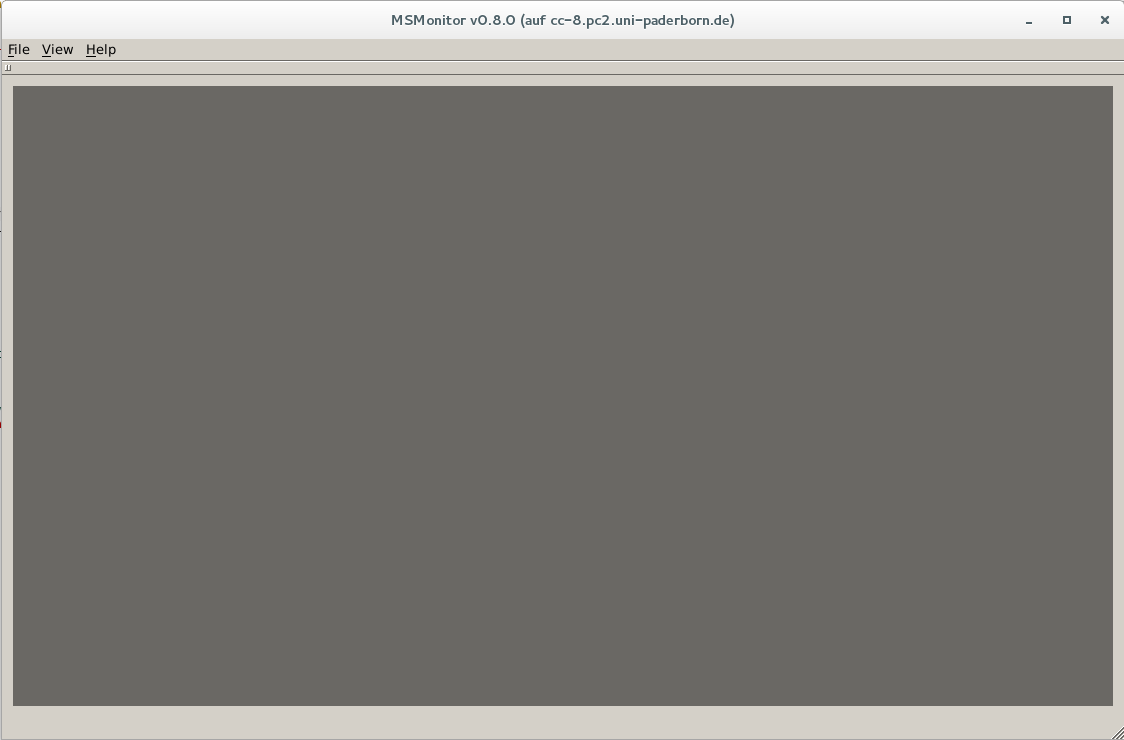
\includegraphics[width=0.9\textwidth]{msm_blank.png} 
		\caption{starting user interface of MSMonitor}
		\label{fig:msm_blank}
	\end{center}
\end{figure}
The settings window and all the plots can be opened from the menu bar or via keyboard shortcuts. They will appear on the mdi area, where they can be moved around according to the user's preference.\newline
The most important window is the settings window, which contains all controls to connect to the server, set up the gui refresh rates and data frequency. This can be seen in \ref{fig:msm_settings}. Tooltips are available for each setting, in order to receive further information.\newline
The settings can be exported to a configuration file, which can also be loaded on the next session, sothat the user does not have to redo the settings each time after starting the program.
\begin{figure}[t!]
	\begin{center}
		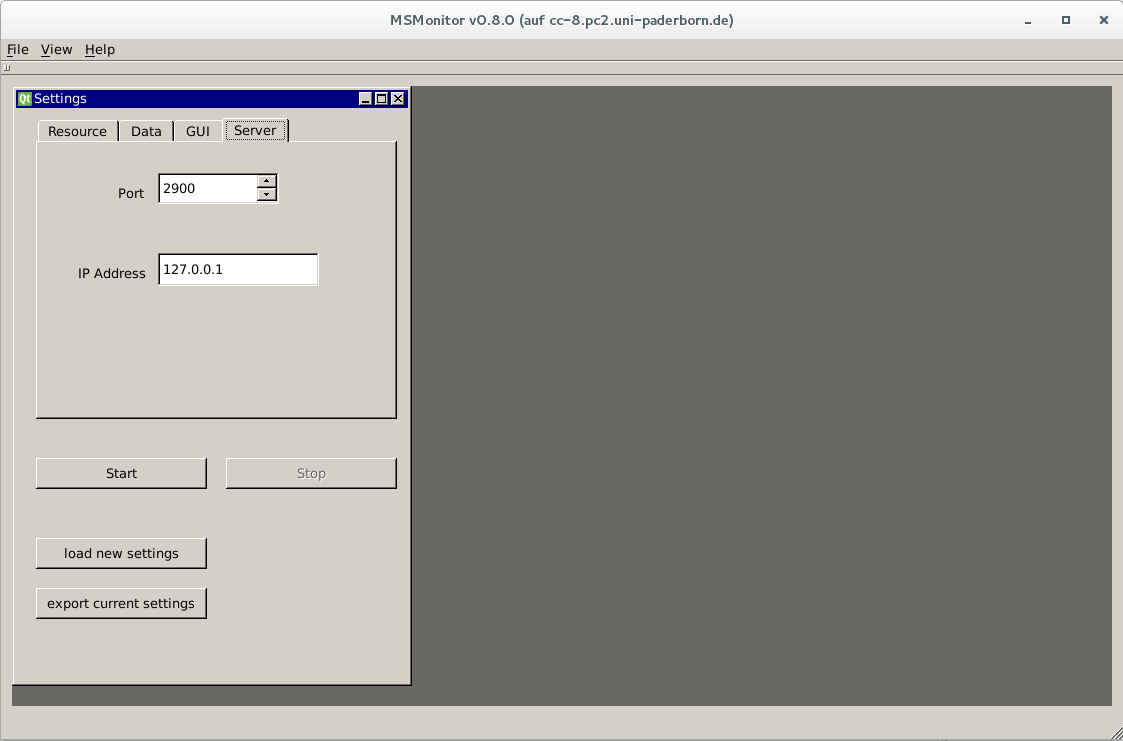
\includegraphics[width=0.9\textwidth]{msm_settings.png} 
		\caption{user interface after enabling the settings window}
		\label{fig:msm_settings}
	\end{center}
\end{figure}
Directly after connecting to the server, the plots will be drawn.\newline 
A plot consists of two tabs. The first tab (plot) contains the coordinate system itself, a legend, a spin box to choose the thickness of the graphs, a screenshot button to export the current graph to png and a csv export button to export the values into a highly manageable comma separated format. This can be seen in \ref{fig:msm_graph}.
\begin{figure}[t!]
	\begin{center}
		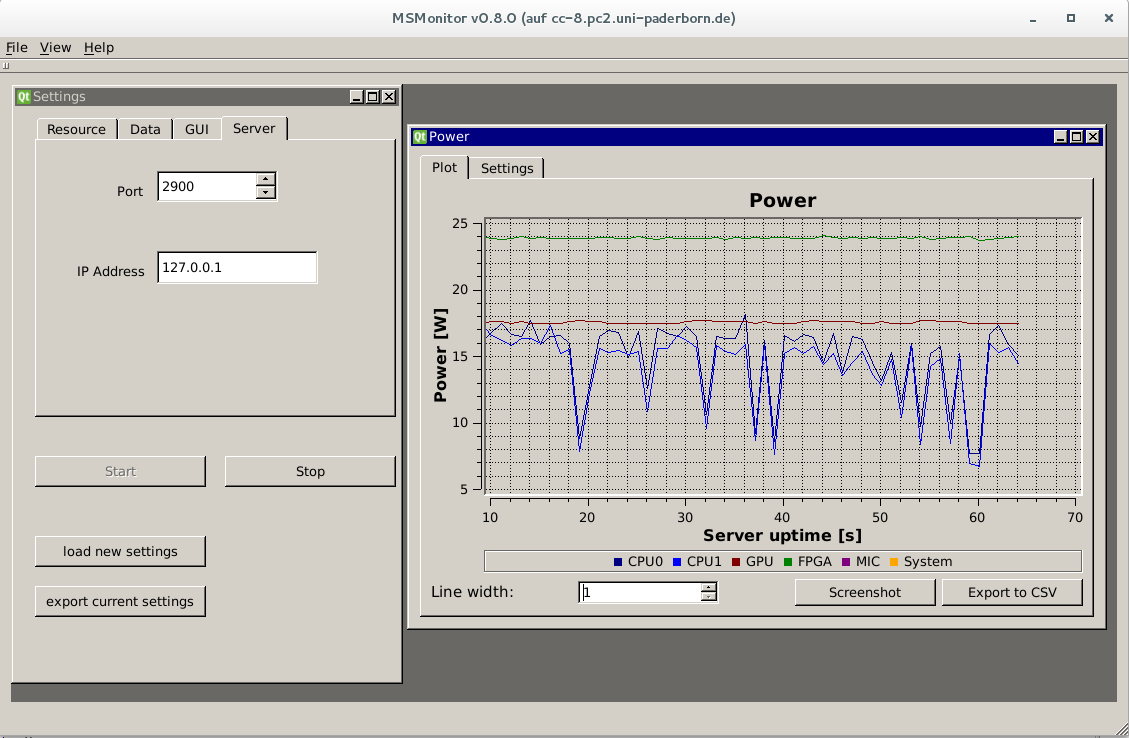
\includegraphics[width=0.9\textwidth]{msm_graph.png} 
		\caption{an active graph in msmonitor}
		\label{fig:msm_graph}
	\end{center}
\end{figure}
The second tab (settings), as shown in \ref{fig:msm_secondTab}, gives the options to remove currently unneeded graphs by simply clicking on the corresponding labels. Recorded global minimum and maximum values are listed next to the labels.\newline
If the graphs have high fluctuation, median and mean filter can be applied over an interval of the user's choice, in order to clarify the tendency of the graph. If the chosen interval is higher than the actual amount of values, nothing will be drawn until the amount of recorded data exceeds the chosen interval.
\begin{figure}[t!]
	\begin{center}
		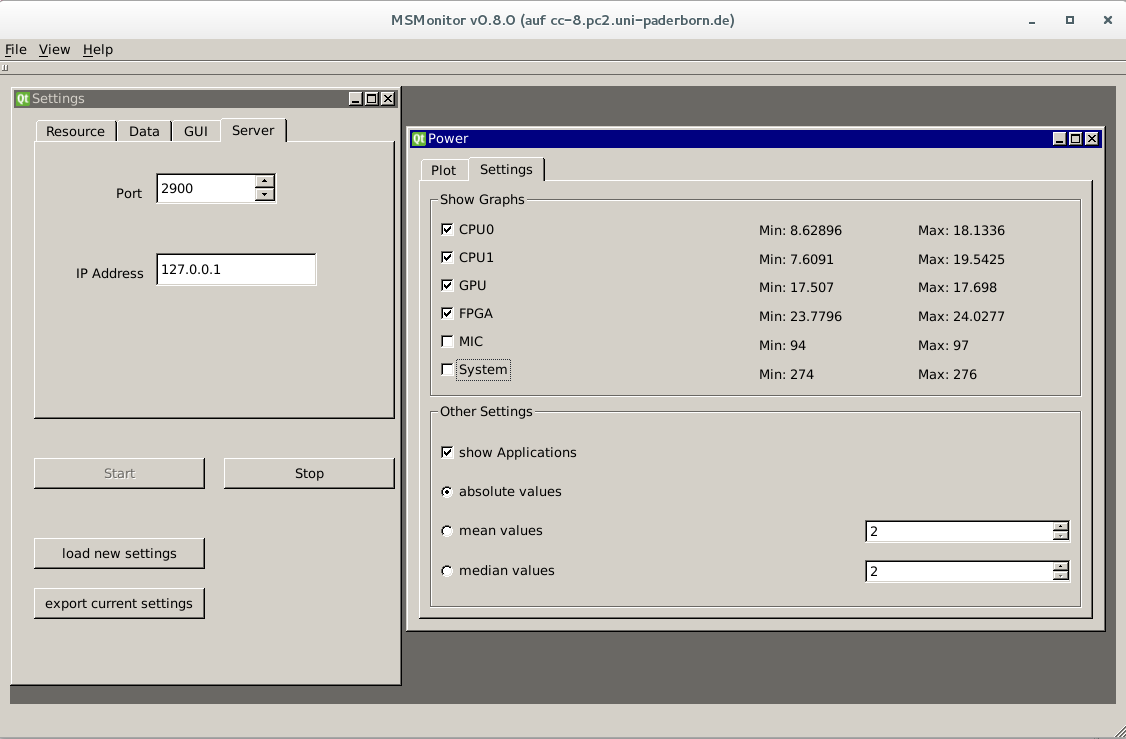
\includegraphics[width=0.9\textwidth]{msm_secondTab.png} 
		\caption{the second tab of a plot}
		\label{fig:msm_secondTab}
	\end{center}
\end{figure}
Besides the option of drawing graphs, start and termination of specific programs can be symbolized on the graphs, by informing the server using the signals SIGUSR1 and SIGUSR2. If an application sends a SIGUSR1 prior to starting, the server informs the clients about a newly started application. Sending a SIGUSR2 to the server, just before terminating the application, makes it inform the clients about a finished application. The unique pid ensures the exclusion of any mix-ups. 



